\documentclass[a4paper]{article}
\newcommand{\sepspace}{\vspace*{1em}}	
%% Language and font encodings
\usepackage[english]{babel}
\usepackage[utf8x]{inputenc}
\usepackage[T1]{fontenc}

%% Sets page size and margins
\usepackage[a4paper,top=3cm,bottom=2cm,left=3cm,right=3cm,marginparwidth=1.75cm]{geometry}

%% Useful packages
\usepackage{amsmath}
\usepackage{graphicx}
\usepackage[colorinlistoftodos]{todonotes}
\usepackage[colorlinks=true, allcolors=blue]{hyperref}


\title{Hydrogen/air ZND detonation}

\author{Emilia Łuczak}
\date{September 2018}

\begin{document}
\maketitle
\sepspace
 \begin{centering}
 METODY KOMPUTEROWE W SPALANIU\\
 \end{centering}
 \sepspace
 \sepspace
 \sepspace
 \sepspace
 \sepspace
 \sepspace
 \sepspace
 \sepspace
 \sepspace
 \sepspace
 \sepspace
 \sepspace
 \sepspace
 \sepspace
 \sepspace
 \sepspace
 \sepspace
 \sepspace
 \sepspace
 \sepspace
 \sepspace
 \sepspace
 \sepspace
 \sepspace
 \sepspace
 \sepspace
 \sepspace
 \sepspace
 \sepspace
 \sepspace
 \sepspace
 \sepspace
 \sepspace
 \sepspace
 \sepspace
 \sepspace
 \sepspace
 \sepspace
 \sepspace
 \sepspace
 \sepspace
 \sepspace
 \sepspace
 \sepspace
 \sepspace
 
 
 \begin{centering}
 Napędy Lotnicze\\
 \end{centering}
 \begin{centering}
 Wydział Mechaniczny Energetyki i Lotnictwa\\
 \end{centering}


\pagebreak
\section{Introduction}

This paper will be dedicated to the ZND detonation of a hydrogen-air mixture. The simulation was run with MATLAB program using Cantera 2.4 and Shock \& Detonation Toolbox. It enabled to analyze a number of characteristics, such as temperature, pressure, density and velocity as functions of initial pressure, initial temperature and equivalence ratio.

\sepspace
\sepspace
\section{ZND Detonation}

\subsection{Model}

The ZND detonation model is a one-dimensional steady model, which can be expressed by an algebraic - differential system of equations. A detonation is a supersonic combustion wave in which a shock wave and a reaction zone are coupled. The leading shock raises the temperature and pressure of a mixture of fuel and oxidizer initiating a coupled thermal branching-chain explosion. In this model, a frozen shock is followed by a finite reaction zone. State 1 is a cold mixture of reactants, state 2 is a shocked (hot) mixture of the same reactants and state 3 is the equilibrium state of the reactive mixture. This model assumes that the composition does not change between states 1 and 2 and they are connected by frozen shock wave. \\

\begin{figure}[h!]
\centering
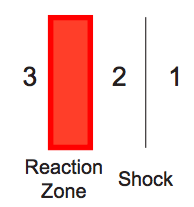
\includegraphics[scale = 1]{01.png}
\caption{\label{fig:1}Cartoon of the ZND detonation model. From source [2]}
\end{figure}
\\

\noindent
It is worth to notice that ZND is a case of Chapman-Jouguet (CJ) detonation. Detonation wave is a shock wave in a reactive medium that is sustained by energy released in chemical reactions that the shock itself triggers and sustains. In CJ theory, it is assumed that chemical reactions take place instantaneously inside the shock. The reaction products are assumed to flow at a locally sonic speed relative to the shock, which is called the Chapman-Jouguet condition.\\

\pagebreak

\subsection{Chemical equation}


In order to find an equivalence ratio, following equation is needed:

\[{2H_2 +(O_2+3,76N_2) }
      = 2H_2O\] 
\\
That simply means there is 91.2g of oxidizer needed for 4g of fuel. It is necessary to achieve the stoichiometric condition - that is $\Phi = 1$. Fuel-air ratio is therefore equal to $4/91.2.4=0.04386$.

\sepspace
\sepspace
\subsection{Shock \& Detonation Toolbox}

SDToolbox is a collection of numerical routines that enables the solution of standard problems for gas-phase explosions using realistic thermochemistry and detailed chemical kinetics. The SD Toolbox employs Cantera software for the chemistry functionality and uses either MATLAB or Python for scripting.\\
The newest toolbox updated in 2014 is compatible with Cantera 2.1. Considering the fact that Cantera 2.4 version was used for computations, some code adjustment was necessary. That is why for objects represating phases $importPhase$ was replaced with $Solution$ where it occured.\\

\sepspace

\section{Results}

Parameters were calculated for different cases as  a function of initial pressure, initial temperature and equivalence ratio. Program displays exact initial conditions for each case.  All results are shown in the form of charts. Following parameters were computed: \\
\bullet $ Post CJ state temperature$\\
\bullet $ Post CJ state pressure$\\
\bullet $ Post CJ state density$\\
\bullet $ CJ velocity$\\
\bullet $ Frozen shock temperature for ZND detonation$\\
\bullet $ Final Temperature for ZND detonation$\\

\noindent
Calculations were run 20 times for each changing parameter. That gives 60 calculated cases in total.

\pagebreak


\subsection{Initial pressure}
\sepspace

Initial pressure vary in the range of 100 000 Pa and 1 000 000 Pa.\\
Initial temperature $T0 = 300$ K\\
Equivalence ratio $\Phi = 1$

\begin{figure}[h!]
\centering
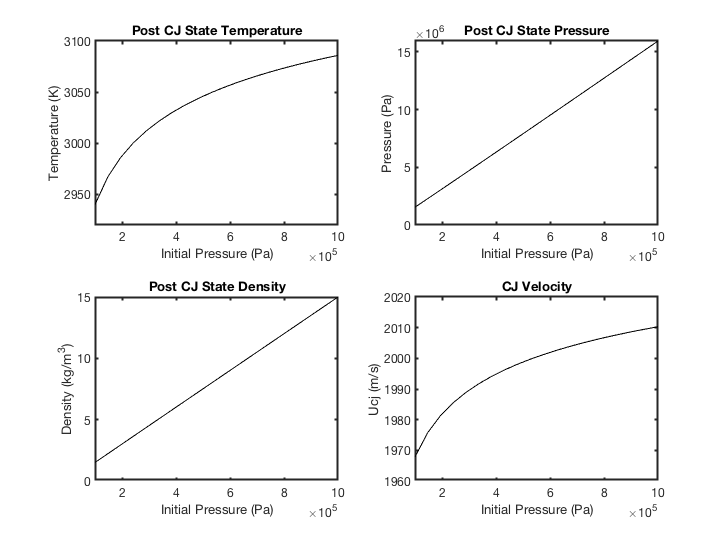
\includegraphics[width=1\textwidth]{P.png}
\caption{\label{fig:1}Parameters as a function of initial pressure.}
\end{figure}

\sepspace

\noindent
\circ $ Post CJ state temperature$\\ 
\indent $- increases with increasing pressure, increase is getting smaller.$\\
\circ $ Post CJ state pressure$\\
\indent $-linearly increase with increasing pressure.$\\
\circ $ Post CJ state density$\\
\indent $- linearly increase with increasing pressure.$\\
\circ $ CJ velocity$\\
\indent $- increase with increasing pressure, increase is getting smaller.$\\



\pagebreak

\subsection{Initial temperature}
\sepspace


Initial temperature vary in the range of 300 K and 1500 K.\\
Initial pressure $P0 = 100 000$ Pa\\
Equivalence ratio $\Phi = 1$

\begin{figure}[h!]
\centering
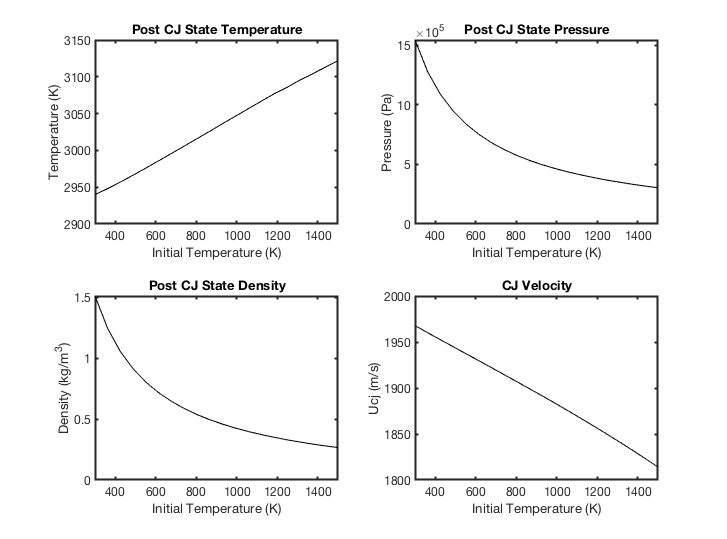
\includegraphics[width=1\textwidth]{T.png}
\caption{\label{fig:1}Parameters as a function of initial temperature.}
\end{figure}


\noindent
\circ $ Post CJ state temperature$\\ 
\indent $- linearly increases with increasing temperature.$\\
\circ $ Post CJ state pressure$\\
\indent $- decreases with increasing temperature, decrease is getting smaller.$\\
\circ $ Post CJ state density$\\
\indent $- decreases with increasing temperature, decrease is getting smaller.$\\
\circ $ CJ velocity$\\
\indent $- linearly decreases with increasing temperature.$\\

\pagebreak

\subsection{Equivalence ratio}
\sepspace

Equivalence ratio vary in the range of 0.5 and 2.\\
Initial pressure $P0 = 100 000$Pa\\
Initial temperature $T0 = 300$ K

\begin{figure}[h!]
\centering
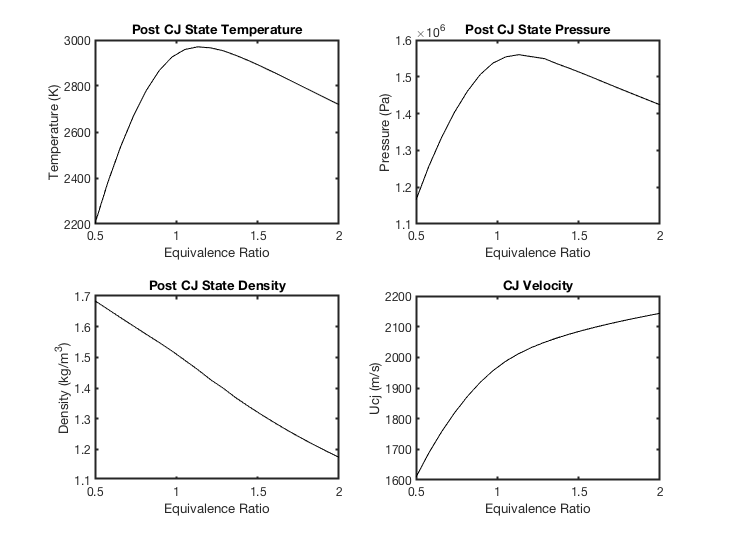
\includegraphics[width=1\textwidth]{F.png}
\caption{\label{fig:1}Parameters as a function of equivalence ratio.}
\end{figure}

\noindent
\circ $ Post CJ state temperature$\\ 
\indent $- increases with increasing equivalence ratio until $\Phi = 1$, then decrease. $\\
\circ $ Post CJ state pressure$\\
\indent $- increases with increasing equivalence ratio until $\Phi = 1$, then decrease. $\\
\circ $ Post CJ state density$\\
\indent $- almost linearly decreases with increasing equivalence ratio$\\
\circ $ CJ velocity$\\
\indent $- increases rapidly with increasing equivalence ratio until $\Phi = 1$, then increase slower. $\\


\pagebreak

\subsection{ZND temperature}
\sepspace

Calculations of frozen shock temperature and final temperature. Calculations were run for all 60 cases described as above. There are 6 charts as a result.

\begin{figure}[h!]
\centering
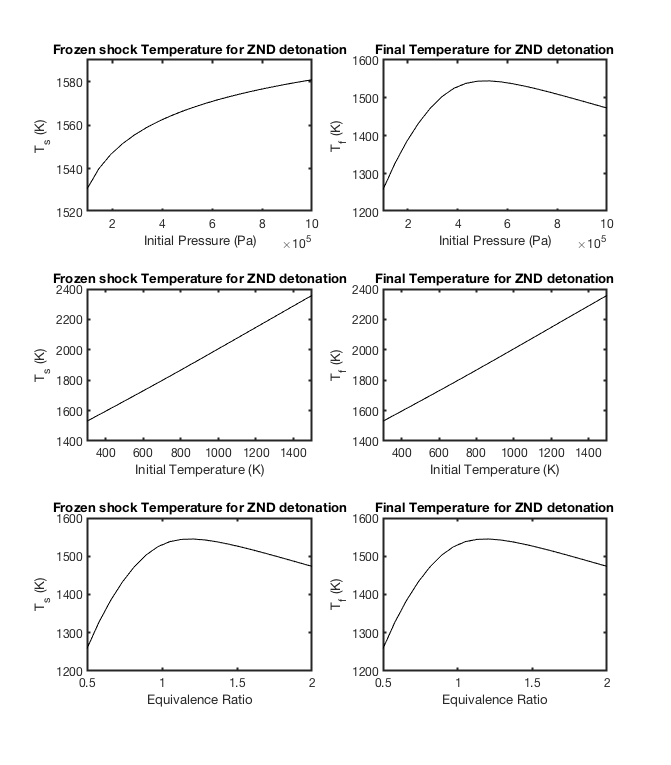
\includegraphics[width=1\textwidth]{ZND.png}
\caption{\label{fig:1}Frozen shock temperature and final temperature for ZND detonation.}
\end{figure}

\noindent
Characteristics of frozen shock temperature and final temperature are almost the same. Temperature increase with increasing temperature and is the highest for $\Phi = 1$/. For initial pressure characteristics are not identical,  frozen shock temperature increase with increasing pressure and final temperature is the highest for 500 000 Pa.


\pagebreak

\section{Conclusions}

Results are probable and close to the real research data. As easy to predict, the highest temperature and pressure occured for equivalence ratio $\Phi = 1$. We can notice a linear relationship between state pressure and initial pressure; state density and initial pressure; state temperature and initial temperature. Interesting thing is that characteristics of frozen shock temperature and final shock temperature are very similar to each other. The only difference is noticeable in those parameters as a function of initial pressure.

\sepspace

\sepspace

\sepspace

\section{References}


[1] 
$http://shepherd.caltech.edu/EDL/PublicResources/cantera/html/SD_Toolbox/
$

\noindent
[2] 
$http://shepherd.caltech.edu/EDL/PublicResources/cantera/doc/tex/ShockDetonation/ShockDetonation.pdf
$

\noindent
[3] 
$http://shepherd.caltech.edu/EDL/PublicResources/cantera/doc/tex/CVZND/CVZND.pdf
$

\noindent
[4] 
$http://cantera.org/documentation/docs-2.4/sphinx/html/matlab/importing.html
$

\noindent
[5] 
$http://math.mit.edu/~kasimov/detonation.html
$


\end{document}

